% !Mode:: "TeX:UTF-8"
%!TEX program  = xelatex

%\documentclass[bwprint]{cumcmthesis}
\documentclass[withoutpreface,bwprint]{cumcmthesis} %去掉封面与编号页

\title{基于虚功原理的系泊系统设计与优化}
\tihao{A}
\baominghao{201723003002}
\schoolname{电子科技大学}
\membera{卫佳杰}
\memberb{谢沁余}
\memberc{任彦璟}
\supervisor{覃思义}
\yearinput{2017}
\monthinput{09}
\dayinput{08}

\begin{document}
 \maketitle
\begin{abstract}

\par 本文分析了锚链选型及长度、重物球的质量、浮标的吃水深度、游动区域及钢桶的倾斜角度之间的关系,给出了基于虚功原理的系泊系统设计与优化模型。  
\par 本文引入广义坐标和虚功原理建立了系泊系统达到平衡时的基本模型, 给出了各部件的倾斜角与作用力满足平衡条件时的方程组。通过逐步搜索计算出风速为$12m/s$和$24m/s$时的相关参数,并拟合出锚链形状表达式。当风速为$12m/s$时,浮标的吃水深度为$0.731$米,游动半径为$14.51$米,钢桶的倾斜角度为$1.02°$;当风速为$24m/s$时,浮标的吃水深度为$0.744$米,游动半径为$18.84$米,钢桶的倾斜角度为$3.91°$。

\par 当风速到达$36m/s$时,若采用前一问重物球质量则不满足条件。因此通过基本模型及非线性规划方法求得在钢桶倾斜角小于$5^o$和锚链与海底平面夹角不超过$16^o$的条件下重物球的设计要求下得出重物球质量为$2890kg$时浮标的吃水深度为1.23米、游动半径19.5米、钢桶与垂直方向的倾角$4^o$。
\par 最后,本文考虑近海水流力对整个系泊系统的影响,并通过选择锚链的型号和节数以及重球的质量使得钢桶的倾斜角度、吃水深度、浮动范围尽可能小,为了简化问题,我们采用逐步优化,并查阅相关资料结合实际通讯的相关原理,依据倾斜角度(第一重要)、吃水深度(第二重要)、游动范围(第三重要)的重要程度进行逐步优化,选出合适的锚链型号、节数和重球质量,并控制变量分别分析风力、水流力和水深对锚链形状的影响。

\keywords{系泊系统 \quad 广义坐标 \quad 虚功原理 \quad 非线性规划 }
\end{abstract}
%\tableofcontents
%\newpage

\section{问题重述}

\par 近浅海观测网的传输节点由浮标系统、系泊系统和水声通讯系统组成(如图1所示)。某型传输节点的浮标系统可简化为底面直径2m、高2m的圆柱体,浮标的质量为1000kg。系泊系统由钢管、钢桶、重物球、电焊锚链和特制的抗拖移锚组成。锚的质量为600kg,锚链选用无档普通链环,近浅海观测网的常用型号及其参数在附表中列出。钢管共4节,每节长度1m,直径为50mm,每节钢管的质量为10kg。要求锚链末端与锚的链接处的切线方向与海床的夹角不超过16度,否则锚会被拖行,致使节点移位丢失。水声通讯系统安装在一个长1m、外径30cm的密封圆柱形钢桶内,设备和钢桶总质量为100kg。钢桶上接第4节钢管,下接电焊锚链。钢桶竖直时,水声通讯设备的工作效果最佳。若钢桶倾斜,则影响设备的工作效果。钢桶的倾斜角度(钢桶与竖直线的夹角)超过5度时,设备的工作效果较差。为了控制钢桶的倾斜角度,钢桶与电焊锚链链接处可悬挂重物球。
\begin{figure}[h]
\small
\centering
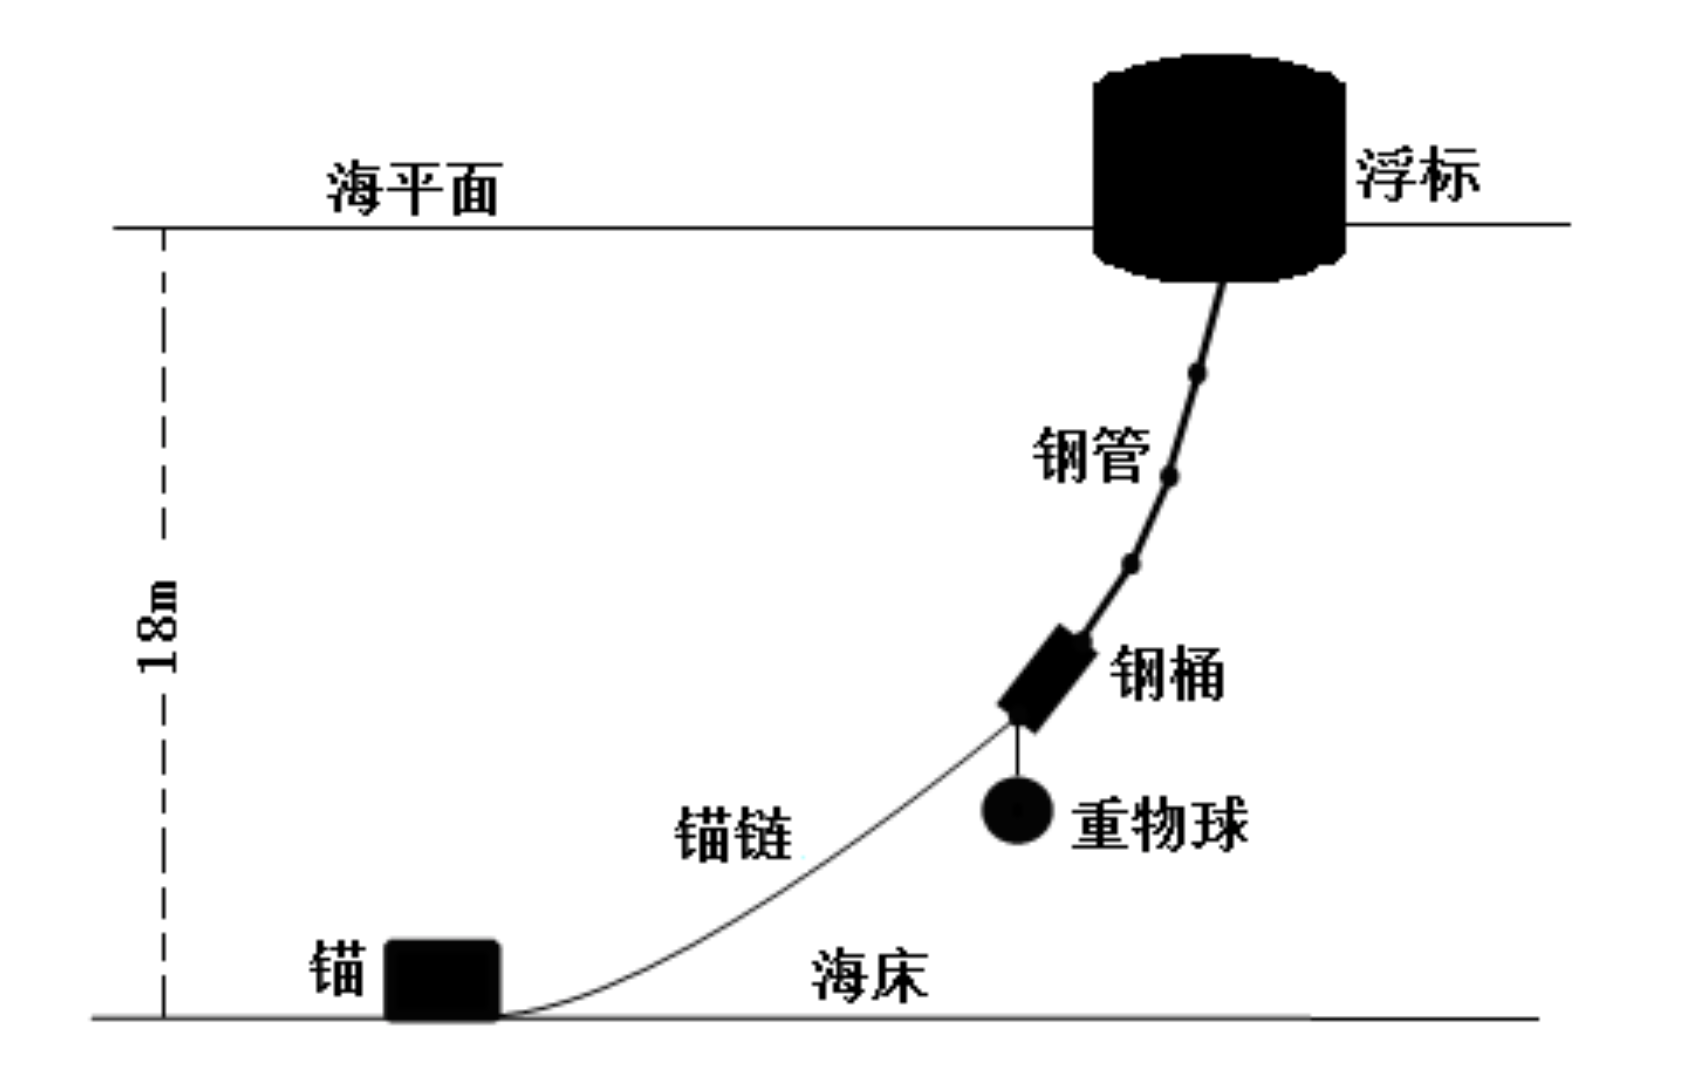
\includegraphics[width=12cm]{wentichongshu.png}
\caption{传输节点示意图} \label{fig:wentichongshu}
\end{figure}
\par 系泊系统的设计问题就是确定锚链的型号、长度和重物球的质量,使得浮标的吃水深度和游动区域及钢桶的倾斜角度尽可能小。

\subsection{问题的提出}
\par 本文需要建立数学模型讨论以下3个问题:
\begin{enumerate}
  \item 在给定的某型传输节点各项相关参数下。若海水静止,分别计算海面风速为$12m/s$和$24m/s$时钢桶和各节钢管的倾斜角度、锚链形状、浮标的吃水深度和游动区域。
  \item 在问题1的假设下,计算海面风速为$36m/s$时钢桶和各节钢管的倾斜角度、锚链形状和浮标的游动区域。调节重物球的质量,使得钢桶的倾斜角度不超过5度,锚链在锚点与海床的夹角不超过16度。
  \item 布放海域的实测水深介于$16m\sim 20m$之间。布放点的海水速度最大可达到$1.5m/s$、风速最大可达到$36m/s$。请给出考虑风力、水流力和水深情况下的系泊系统设计,分析不同情况下钢桶、钢管的倾斜角度、锚链形状、浮标的吃水深度和游动区域。
\end{enumerate}

\section{问题分析}
\par 系泊系统的设计问题就是确定锚链的型号、长度和重物球的质量,使得浮标的吃水深度和浮标的游动区域及钢桶的倾斜角度尽可能小。首先钢桶的倾斜角度直接影响设备的通信效果,倾斜角度越小,通信效果越好;其次查阅的资料,我们可以得到对于浮标的吃水深度越小,则相应的通信效果也越好;而为了达到同样的目的,浮标的游动区域也尽可能小。
\subsection{问题一:已知风速和和钢球质量条件下的系泊系统计算模型}
锚链的型号,长度,重物球质量已知,在特定的风速下整个系统处于稳定状态,本文根据锚链不同的形态与水深的约束关系,得出浮标的吃水深度。我们将锚链视为单个锚链链环的连接组成,得出每个锚链链环、钢桶的倾角,每个杆与水平面的夹角都是固定值,通过分析力学的虚功原理得出每个链环、钢桶、每个钢管与水平方向的夹角大小,通过三者与水平方向的夹角我们可以得出锚链的形状与浮标的游动区域。
\subsection{问题二:风速为$36m/s$时系泊系统优化模型}
当海面风速增大到$36m/s$时,我们需要分析锚链的形状,并与前一问使用相同的方法求解得出每个链环、钢桶、每个钢管与水平方向的夹角大小。求解后比较结果是否满足题中约束条件,如果不满足题中的约束条件,那么对钢球的质量进行搜索,直到钢球的质量,可以使得每个链环、钢桶、每个钢管与水平方向的夹角大小满足约束条件。
\subsection{问题三:风力、水流力和水深综合影响下系泊系统优化模型}
在第一问的基础上,我们需要考虑由于海流速度产生的近海水流力对系统的影响,在第一问模型的基础上需要进行优化,并通过选择锚链的型号和节数以及重球的质量使得钢桶的倾斜角度、吃水深度、浮动范围尽可能小,为了简化问题,我们采用逐步优化,并查阅相关资料结合实际通讯的相关原理,依据倾斜角度(第一重要)、吃水深度(第二重要)、游动范围(第三重要)这样的重要程度进行逐步优化,选出合适的锚链型号与节数和重球质量,最后控制变量分别分析风力、水流力和水深情况对锚链形状的影响。
\section{模型的假设}

\begin{enumerate}
	\item 海底为水平平面。
	\item 风向仅在水平方向上,且风速恒定。
	\item 各个部件之间衔接处绝对光滑。
	\item 各部件均为均质部件。
	\item 不考虑重物球的浮力作用。
	\item 假设浮标始终垂直于海平面。
\end{enumerate}

\newpage
\section{符号说明}

\begin{table}[!h]
\centering
\begin{tabular}{ccc}
\toprule
\makebox[0.2\textwidth][c]{符号}	&  \makebox[0.4\textwidth][c]{意义} &  \makebox[0.2\textwidth][c]{单位} \\
\midrule
$A$& 锚链& (部件名称)\\
$B$& 重物球&(部件名称) \\
$P$& 钢管&(部件名称) \\
$D$& 钢桶& (部件名称)\\
$VAR_f$& 浮标相关量& (角标为$f$的变量)\\
$G$ & 重力(角标用部件名称表示对应变量)& $N$\\
$m$& 质量(角标用部件名称表示对应变量)& $kg$\\
$f$& 浮力(角标用部件名称表示对应变量)& $N$\\
$L$& 总长度(角标用部件名称表示对应变量)& $m$\\
$l_A$& 单节锚链长度& $m$\\
$d$& 直径(角标用部件名称表示对应变量)&$m$ \\
$\rho$& 密度(角标用部件名称表示对应变量)&$kg/m^3$ \\
$F_{wind}$& 风载荷(风力)& $N$\\
$FW$& 近海水流力(角标用部件名称表示对应变量)& $N$\\
$h$& 浮标吃水深度& $m$\\
$H$& 海平面高度& $m$\\
$v$& 海风风速& $m/s$\\
$\mu$& 海水流速& $m/s$\\
$\theta$& 与水平面的夹角(角标用部件名称表示对应变量)& 度\\
$n$& 浮于水中的锚链环个数& 个\\
\bottomrule 
\end{tabular}
\end{table}

\newpage
\section{建模前准备}

\subsection{广义坐标\upcite{理论力学}}
\par 对于n个质点形成的力学体系,如果有k个几何约束
\begin{equation}
	\label{guangyi-1}
	f_\alpha (x,y,z,t) = 0 \qquad (\alpha = 1,2,\cdots,k)
\end{equation}
\par 那么独立坐标就减少$3n-k$个。这些独立坐标,也就是力学体系的坐标。在力学体系只受有几何约束的情形下,这些独立坐标的数目叫做力学体系的\textbf{自由度}。但对于微分约束来讲,自由度的数目则可能小于独立坐标的数目。
\par 既然只有$3n-k$个坐标是独立的,如果我们令$3n-k=s$,那么我们就可以通过公式(\ref{guangyi-1}),将$3n$个不独立的坐标用s个独立参数$q_1,q_2,\cdots,q_s$及$t$表出,即
\begin{equation}
	\label{guangyi-2}
\left. 
  	\begin{array}{lr}  
  	x_i = x_i (q_1,q_2,\cdots,q_s,t)\\
  	y_i = y_i (q_1,q_2,\cdots,q_s,t)\\
  	z_i = z_i (q_1,q_2,\cdots,q_s,t)\\   
	\end{array}  
\right\} \quad (i = 1,2,\cdots,n,s<3n)  
\end{equation}
或
\begin{equation}
	\label{guangyi-3}
	\textbf{r}_i = \textbf{r}_i (q_1,q_2,\cdots,q_s,t) \qquad (i = 1,2,\cdots,n,s<3n)
\end{equation}
\par 公式(\ref{guangyi-3})中$q_1,q_2,\cdots,q_s$叫做拉格朗日\textbf{广义坐标},它不一定是长度,可以是角度或者其他物理量,例如面积$A$、 体积$\tau$、电极化强度$P$、磁化强度$M$等等。在几何约束的情况下,广义坐标的数目和自由度的数目相等。此时$s$个广义坐标,就足以规定力学体系的位置。
\subsection{虚功原理\upcite{理论力学}}
\subsubsection{实位移与虚位移}
\par 设质点按规律(\ref{shiweiyi})
\begin{equation}
	\label{shiweiyi}
	x = f_1(t),\quad y = f_2(t),\quad z = f_3(t)
\end{equation}
运动,那么在无限短的时间$\mathrm{d}t$内,质点的位移为$\mathrm{d} \textbf{r}(\mathrm{d}x,\mathrm{d}y,\mathrm{d}z)$,而且$\mathrm{d} \textbf{r} = \mathop{\textbf{r}}\limits^{\cdot} \mathrm{d}t$,或$\mathrm{d}x = \mathop{x}\limits^{\cdot} \mathrm{d}t$,$\mathrm{d}y = \mathop{y}\limits^{\cdot} \mathrm{d}t$,$\mathrm{d}z = \mathop{z}\limits^{\cdot} \mathrm{d}t$。在这种情形下,质点的位矢$\textbf{r}$或坐标$(x,y,z)$由于参数$t$改变$\mathrm{d}t$而发生变化。如果$\mathrm{d}t = 0$,即时间没有变化,则$\mathrm{d} \textbf{r} = 0$,或$\mathrm{d}x= \mathrm{d}y= \mathrm{d}z=0$。质点由于运动实际上所发生的位移叫做\textbf{实位移},并以$\mathrm{d} \textbf{r}$表示。
\par 假设某一时刻$t$,质点$P$在约束所许可的情况下,发生了一个无限小的变更。这一变更,不是由于质点的运动而实际发生的。而只是想象中可能发生的位移,它只决定于质点在此时刻的位置和加在它上面的约束,而不是由于时间改变而引起的。这种位移叫做\textbf{虚位移},并以$\delta \textbf{r}$表之。由于时间$t$没有改变,故$\delta t =0$。一般来讲,在任一时刻$t$,在约束许可的情况下,质点的虚位移可以不止一个。
\subsubsection{理想约束}
\par 作用在质点上的力(包括约束反力)$F$在任意虚位移$\delta \textbf{r}$中所做的功,叫做\textbf{虚功},如果作用在一力学体系上诸约束反力在任意虚位移$\delta \textbf{r}$中所作的虚功之和为零,即
\begin{equation}
	\label{lixiangyueshu}
	\sum\limits_{i=1}^{n} \textbf{R}_i \cdot \delta \textbf{r}_i = 0
\end{equation}
那么这种约束叫做\textbf{理想约束}。光滑面、光滑曲线、光滑铰链、刚性杆、不可伸长的绳等都是理想约束。引入虚位移的目的,就在于利用公式(\ref{lixiangyueshu})来消去这些约束反力。

\subsubsection{虚功原理}
\par 以下只讨论不可解约束的情况。设受有$k$个几何约束的某力学体系处于平衡状态,取体系中任一质点$\textbf{P}_i$,并设作用在此质点上主动力的合力为$\textbf{F}_i$,约束反力的合力为$\textbf{R}_i$,则因在此体系中每一质点都必须处于平衡状态中,故此时必有
\begin{equation}
	\label{xugong-1}
	\textbf{F}_i + \textbf{R}_i = 0 \qquad (i = 1,2,\cdots,n)
\end{equation}
\par 现让每一质点自它的平衡位置发生一虚位移$\delta \textbf{r}_i$,则由公式(\ref{xugong-1}),得
\begin{equation}
	\label{xugong-2}
	\textbf{F}_i \cdot \delta \textbf{r}_i+ \textbf{R}_i \cdot \delta \textbf{r}_i = 0 \qquad (i = 1,2,\cdots,n)
\end{equation}
把公式(\ref{xugong-2})中各等式相加,就得到
\begin{equation}
	\label{xugong-3}
	\sum\limits_{i=1}^{n} \textbf{F}_i \cdot \delta \textbf{r}_i+ \sum\limits_{i=1}^{n} \textbf{R}_i \cdot \delta \textbf{r}_i = 0 \qquad (i = 1,2,\cdots,n)
\end{equation}
但如为理想约束,则根据公式(\ref{lixiangyueshu}),$\sum\limits_{i=1}^{n} \textbf{R}_i \cdot \delta \textbf{r}_i = 0$,因此,如果这样的力学体系处于平衡状态,则其\textbf{平衡条件}是
\begin{equation}
	\label{xugong-4}
	\delta W = \sum\limits_{i=1}^{n} \textbf{F}_i \cdot \delta \textbf{r}_i = 0
\end{equation}
或
\begin{equation}
	\label{xugong-5}
	\delta W = \sum\limits_{i=1}^{n} (\textbf{F}_{ix} \delta x_i + \textbf{F}_{iy} \delta y_i + \textbf{F}_{iz} \delta z_i) = 0
\end{equation}
\par 反之,也可以证明,如果平衡位置是约束所允许的位置,则当公式(\ref{xugong-4})对任意$\delta \textbf{r}_i$都成立时,系统在该位置必保持平衡。由此可知,受有理想约束的力学体系平衡的充要条件是此力学体系的诸主动力在任意虚位移中所做的元功之和等于零。该关系叫做\textbf{虚功原理},也叫\textbf{虚位移原理}。
\newpage
\section{已知风速和和钢球质量条件下的系泊系统计算模型}
\subsection{模型建立}
\par 通过虚功原理建立基于分析力学的计算模型,将锚链的每一个链环、重物球、钢桶、四节钢管、浮标视为单独个体进行分析,最终分别求得风速为12$m/s$和24$m/s$时系泊系统的各个状态描述参数。

\par 本文分别用$f$表示浮标,$P_j$表示钢管第$j$节钢管,$D$表示钢桶, $A_k$表示锚链第$k$节锚链,$B$表示重物球。在这里,本文所考虑的主动力包括:近海面风力Ff,每个部件的重力(用$G$和部件的标号作下标表示), 海水对整个系统中各个组件的浮力(用$F$和部件的标号作下标表示)。每个部件所受主动力及建立坐标系如图(\ref{fig:zuobiaoxi})所示。

\begin{figure}[!htpb]
\small
\centering
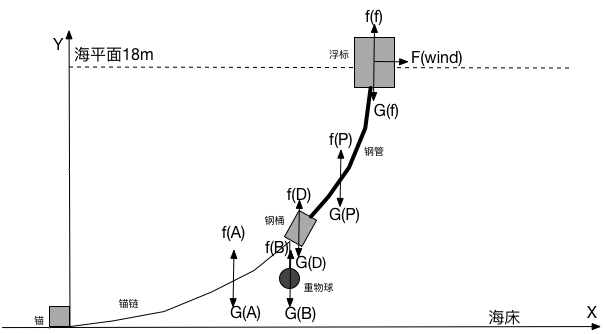
\includegraphics[width=\textwidth]{zuobiaoxi.png}
\caption{坐标系建立} \label{fig:zuobiaoxi}
\end{figure}
\subsubsection{根据几何关系建立各组件重心与倾角关系}
\par 在广义坐标系中,我们给出各个部件的重心位置和该部件与海平面间夹角的几何关系表达式如下公式(\ref{weiyifangcheng-1})所示。其中,用$y$加部件标号作为对应部件的$y$轴坐标位置,$x$加部件标号作为对应部件的$x$轴坐标位置。用$\theta$加部件标号表示该部件与海平面间夹角。
\begin{equation}
	\label{weiyifangcheng-1}
	\left\{
	\begin{array}{lr}
		y_{A1} = \frac{l_A}{2} sin \theta_{A1}\\
		y_{A2} = \frac{l_A}{2} sin \theta_{A2} + l_A sin \theta_{A1}\\
		\cdots \\
		y_{An} = \frac{l_A}{2} sin \theta_{An} + \sum\limits_{i=1}^{n-1} l_A sin \theta_{Ai}\\
		y_B = \sum\limits_{i=1}^{n} l_A sin \theta_{Ai}\\
		y_D = \frac{l_D}{2} sin \theta_D + \sum\limits_{i=1}^{n} l_A sin \theta_{Ai}\\
		y_{P1} = \frac{l_P}{2} sin \theta_{P1} + l_D sin \theta_D + \sum\limits_{i=1}^{n} l_A sin \theta_{Ai}\\
		\cdots \\
		y_{P4} = \frac{l_P}{2} sin \theta_{P4} + \sum\limits_{i=1}^{3} l_P sin \theta_{Pi} + l_D sin \theta_D + \sum\limits_{i=1}^{n} l_A sin \theta_{Ai}\\
		x_f = \sum\limits_{i=1}^{4} l_P cos \theta_{Pi} + l_D cos \theta_D + \sum\limits_{i=1}^{n} l_A cos \theta_{Ai} + \frac{1}{2} d_f + (N - n) \cdot l_A\\
		y_f = \sum\limits_{i=1}^{4} l_P sin \theta_{Pi} + l_D sin \theta_D + \sum\limits_{i=1}^{n} l_A sin \theta_{Ai} + \frac{1}{2} L_f\\
	\end{array}
	\right.
\end{equation}

\par 公式组(\ref{weiyifangcheng-1})中,$y_{Ai}$为第$i$节锚链环重心所在的纵坐标,其中$l_A$为题中所给出的第二型锚链的单节链环的长度,$\theta_{Ai}$为第$i$节锚链环与$x$轴正方向(平行于海平面)的夹角;$y_B$为金属球的球心纵坐标,可以用最后一节锚链链环的纵坐标代替;$y_D$为金属圆桶中心的纵坐标,为金属圆桶轴线与$x$轴正方向的夹角;$y_f$为浮标重心所在的纵坐标,$L_f$为浮标的高度,$d_f$为浮标的直径,$x_f$为浮标重心所在的横坐标。
\par 通过分析,我们添加如公式(\ref{y-yueshu-1})所示的约束条件,保证所有链环、钢管、钢桶在竖直方向上的投影和浮标的吃水深度($h$)之和为18$m$。
\begin{equation}
	\label{y-yueshu-1}
	\sum\limits_{i=1}^{4} l_P sin \theta_{Pi} + l_D sin \theta_D + \sum\limits_{i=1}^{n} l_A sin \theta_{Ai} + h = 18
\end{equation}

\subsubsection{各部件所受主动力的分析}
\par 对于单个锚链链环,受到自身重力与海水对其的浮力两个主动力,其合力可由公式()求得。其中 为锚链单位长度的质量。
\begin{equation}
	\label{q1-pa}
	P_A = f_A - G_A  = \rho_w \cdot g \cdot \frac{\lambda_A \cdot l_A}{\rho_A} - \lambda_A \cdot l_A \cdot g
\end{equation}
\begin{equation}
	\label{q1-pd}
	P_D = f_D -G_D = \rho_w \cdot g \cdot (\frac{d_D}{2})^2 \pi \cdot L_D - m_D \cdot g
\end{equation}
\begin{equation}
	\label{q1-pp}
	P_P = f_P -G_P = \rho_w \cdot g \cdot (\frac{d_P}{2})^2 \pi \cdot L_P - m_P \cdot g
\end{equation}
\begin{equation}
	\label{q1-wind}
	F_{wind} = 0.625 \times S v^2
\end{equation}
\par 与单个锚链链环相似,对于钢桶竖直方向有合力$P_D$如公式(\ref{q1-pd})所示;对于钢管竖直方向有合力$P_P$如公式(\ref{q1-pp})所示;对于金属球,由于浮力对于密致金属球影响极小,因此忽略其所受到的浮力,金属球所受合力$P_B$直接由其重力表示为$P_B = G_B = m_B \cdot g$;风载荷(风力)$F_{wind}$的定义如公式(\ref{q1-wind})所示,其中$S$为迎风面积、$v$为风速。
\subsubsection{基于虚功原理的计算}

\par 对于整个系泊系统,当系统达到稳定时,可以认为该系统处于一个受理想约束的力学体系中,在该体系中,所有的主动力的任意虚位移所作的所有元功之和等于零,由此得到系泊系统的平衡方程(\ref{q1-xugonyuanli})。

\begin{equation}
	\label{q1-xugonyuanli}
	\sum\limits_{i=1}^{n} P_A \cdot \delta y_{Ai} + P_D\cdot \delta y_D + \sum\limits_{i=1}^{4}P_P\cdot \delta y_{Pi} + P_B \cdot \delta y_{B} + P_f \cdot \delta y_{f} + F_{wind} \cdot \delta x_f = 0
\end{equation}

\par 在公式(\ref{q1-xugonyuanli})中,$P_A$、$P_D$、$P_P$、$P_B$、$P_f$分别表示锚链、钢桶、钢管、钢球和浮标竖直方向所受到的力,$F_{wind}$表示水平风载荷。$\delta y_{Ai}$、$\delta y_{Di}$、$\delta y_{Pi}$、$\delta y_{B}$、$\delta y_{f}$、$\delta y_{Xf}$、表示系统内各个部件分别的虚位移。
\par 将公式(\ref{q1-xugonyuanli})展开并将公式组(\ref{weiyifangcheng-1})中各个变量的计算公式代入得虚功原理计算方程如公式(\ref{q1-xugong-zhankai})所示。
\begin{equation}
	\label{q1-xugong-zhankai}
	\begin{split}
		0 &= \left[ P_A \cdot \delta(\frac{l_A}{2}sin \theta_{A1}) + P_A \cdot \delta(\frac{l_A}{2}sin \theta_{A2} + l_A sin \theta_{A1}) + \cdots +P_A \cdot \delta(\frac{l_A}{2}sin \theta_{An} + \sum\limits_{i=1}^{n-1} l_A sin \theta_{Ai}) \right] \\ 
		& + P_D \cdot (\frac{l_D}{2}sin \theta_{D} + \sum\limits_{i=1}^{n}l_A sin \theta_{Ai}) + \left[ {P_P \cdot \delta(\frac{l_P}{2}sin \theta_{P1} + l_D sin \theta_D + \sum\limits_{i=1}^{n}l_A sin\theta_{Ai} ) + \cdots} \right. \\
		& \left. {+ P_P \cdot \delta(\frac{l_P}{2}sin \theta_{P4} + \sum\limits_{i=1}^{3} l_P sin \theta_{Pi} +l_D sin \theta_D \sum\limits_{i=1}^{n}l_A sin\theta_{Ai} )} \right] + P_B \cdot \delta (\sum\limits_{i=1}^{n} l_A sin \theta_{Ai}) + \\
		& P_f \cdot \delta (\sum\limits_{i=1}^{4}l_P cos\theta_{Pi} + l_D sin \theta_{D} \sum\limits_{i=1}^{n}l_A sin \theta_{Ai} + \frac{1}{2}L_f) + F_{wind} \cdot \left({\sum\limits_{i=1}^{4}l_P cos \theta_{Pi} + l_D cos \theta_D +} \right. \\
		& \left. {\sum\limits_{i=1}^{n}l_A cos \theta_{Ai} + (n-1)l_A + \frac{1}{2} d_f} \right)
	\end{split}
\end{equation}
\par 将上述公式(\ref{q1-xugong-zhankai})进行化简可得到如下公式(\ref{q1-xugong-huajian})
\begin{equation}
	\label{q1-xugong-huajian}
	\begin{split}
		0 &= l_A \sum\limits_{i=1}^{n} \left\{ { \left[(n+\frac{1}{2} - i)P_A +P_D +4P_P +P_B+P_f\right]cos \theta_{Ai} - F_{wind}sin\theta_{Ai} }\right\} \cdot \delta\theta_{Ai} + \\
		& l_D \left[ {(\frac{1}{2} P_D +4P_P+P_f)cos\theta_D - F_{wind}sin\theta_D }\right] \cdot \delta \theta_D  + \sum\limits_{i=1}^{4}l_P \left[ {(P_P(4.5-i)+P_f)cos\theta_{Pi}}\right.\\
		& \left. {-F_{wind} sin\theta_{Pi} }\right] \cdot \delta \theta_{Pi}
	\end{split}
\end{equation}
\par 由公式(\ref{q1-xugong-huajian})可以推出部件总数个方程用于求解,通过虚功原理可以得出$\delta \theta_{Ai}$、$\delta \theta_{D}$、$\delta \theta_{Pi}$是相互独立的,因此可令$\delta \theta_{Ai}$、$\delta \theta_{D}$、$\delta \theta_{Pi}$之前的系数为零,得到如下公式组(\ref{q1-xugong-qiujie}),为了简化表述,将相似方程通过循环变量$i$的形式表示。
\begin{equation}
	\label{q1-xugong-qiujie}
	\left\{
	\begin{split}
		& \left[ (n + \frac{1}{2} - i)P_A +P_D+4P_P+P_B+P_f \right] cos\theta_{Ai} - F_{wind} sin\theta_{Ai} = 0\\
		& (\frac{1}{2} P_D+4P_P+P_f)cos\theta_D - F_{wind}sin\theta_{D} = 0\\
		& \left[ P_P(4.5-i)+P_f \right] cos\theta_{Pi} - F_{wind} sin \theta_{Pi}\\
	\end{split}
	\right.
\end{equation}
由公式组(\ref{q1-xugong-qiujie})各个方程可解得系泊系统中任意部件与海平面的夹角$\theta$的表达式(\ref{q1-xugong-qiujie-2})。其中$\theta_{Ai}$为不落于海床上的第$i$节锚链环与海平面间的夹角,$\theta_D$为钢桶轴线与水平方向的夹角,$\theta_{Pi}$为第$i$节钢管于海平面的夹角。
\begin{equation}
	\label{q1-xugong-qiujie-2}
	\left\{
	\begin{split}
		& \theta_{Ai} = arctan\frac{(n + \frac{1}{2} - i)P_{Ai} +P_D+4P_P+P_B+P_f}{F_{wind}} \\
		& \theta_D = arctan\frac{\frac{1}{2}P_D+4P_P+P_f}{F_{wind}}\\
		& \theta_{Pi} = arctan\frac{P_P(4.5-i)+P_f}{F_{wind}}\\
	\end{split}
	\right.
\end{equation}
将公式组(\ref{q1-xugong-qiujie-2})中各个$\theta$的计算公式代入约束方程(\ref{rey-yueshu-1})中进行求解,得到最终结果。
\begin{equation}
	\label{rey-yueshu-1}
	\sum\limits_{i=1}^{4} l_P sin \theta_{Pi} + l_D sin \theta_D + \sum\limits_{i=1}^{n} l_A sin \theta_{Ai} + h = 18
\end{equation}
\subsection{模型求解}
\par 在第一问中,锚链选择长度为$22.05m$的II型电焊锚链(锚链链环个数为210个),选用$1200kg$的重物球。求解的海域内海水密度为$1.025×10^3kg/m^3$。

\subsubsection{海风风速为$12m/s$时的求解}

\par 当海上的风速为$12m/s$时,假设$210$个锚链链环均不沉于海床面上,通过模型解得锚链,钢桶,钢管在竖直方向上的投影高度大于$18$米,不符合实际。因此$210$个锚链链环中一定有一部分锚链沉于海床面上。由于第一节锚链一定在海底,因此第一节锚链与水平方向的夹角为$0^o$。

\begin{equation}
	\label{q1-ans-1}
	\theta_{A1} = arctan\frac{(n + \frac{1}{2} - i)P_{A1} +P_D+4P_P+P_B+P_f}{F_{wind}} = 0 
\end{equation}
\par 由公式(\ref{q1-ans-1})可以求解出,此时的浮标吃水深度$h$为$0.73072$米。
\par 通过改变浮于海水中锚链链环的个数,使得锚链、钢桶、钢管在竖直方向上的投影高度等于18米。最终确定浮于海水中的锚链环的个数为$147$个(有$6.615m$的锚链沉于海床面上)。
\par 计算得到锚链、钢桶、钢管的重心坐标,得到系泊系统中各个部件的位置如下图(\ref{fig:q1-12-1})所示。
\begin{figure}[h]
\small
\centering
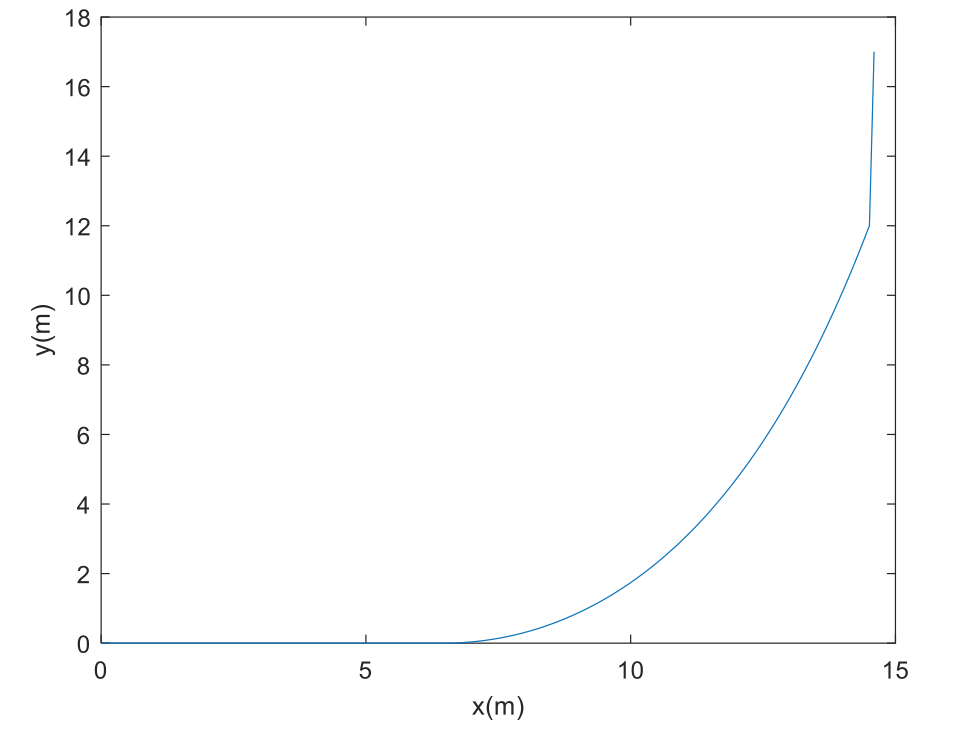
\includegraphics[width=12cm]{q1-12-1.png}
\caption{风速为$12m/s$时系泊系统各组件位置} \label{fig:q1-12-1}
\end{figure}
\par 由于在靠近锚的一侧有部分锚链环沉在海床面上,为了提高拟合精准度,将锚链重心连线分段拟合,得到锚链的拟合曲线如公式(\ref{q1-ans-2})所示。
\begin{equation}
	\label{q1-ans-2}
	\left\{
\begin{aligned}
y & = 0& 	0<x<6.5100\\
y & = 0.000052x^5-0.0015x^4+0.019x^3-0.021x^2-1.02x+ 4.23 &  	6.5100\leqslant x<14.5085\\
\end{aligned}
\right.
\end{equation}
\par 经检验,拟合标准差在$10^{-3}$数量级,因此上述的拟合结果较为精确。
\par 我们认为浮标的游动距离为浮标的平衡位置与锚所在位置的水平距离。求解出当风速为$12m/s$时浮标的游动范围为以锚为圆心半径为$14.5058$米的圆。当风向沿$x$轴正方向时,锚链形状如图(\ref{fig:q1-12-2})所示。
\begin{figure}[h]
\small
\centering
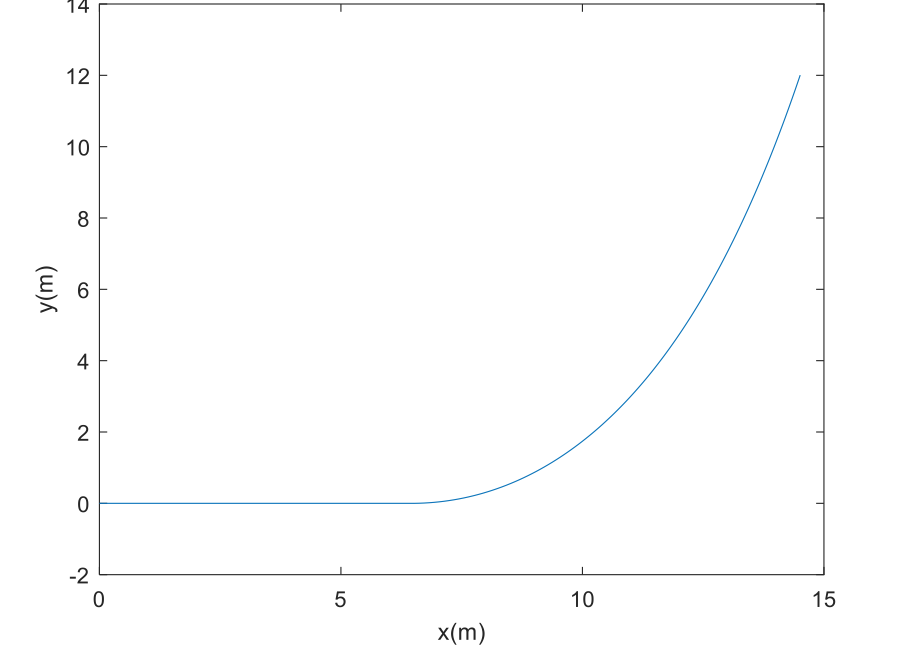
\includegraphics[width=12cm]{q1-12-2.png}
\caption{风速为$12m/s$时锚链形状拟合曲线} \label{fig:q1-12-2}
\end{figure}
\newpage
\subsubsection{海风风速为$24m/s$时的求解}
\par 当海上的风速为$24m/s$时,假设$210$个锚链链环均不沉于海床面上,通过模型解得锚链,钢桶,钢管在竖直方向上的投影高度小于$18$米,符合实际。因此$210$个锚链链环均浮于海水中。通过对浮标吃水深度$h$精确到$0.001$米的搜索,得出在$0.74432$米的吃水深度下,锚链、钢桶、钢管在竖直方向上的投影高度与浮标吃水深度之和满足水深18米的约束。


\par 与风速为$12m/s$时形同的方式,计算得到锚链、钢桶、钢管的重心坐标,得到系泊系统中各个部件的位置如下图(\ref{fig:q1-24-1})所示。
\begin{figure}[h]
\small
\centering
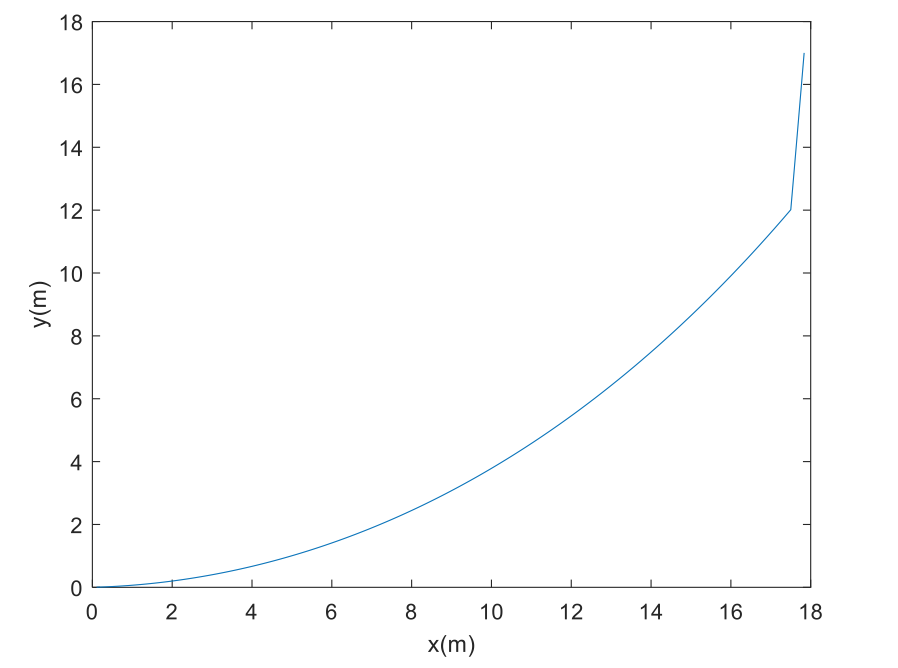
\includegraphics[width=12cm]{q1-24-1.png}
\caption{风速为$24m/s$时系泊系统各组件位置} \label{fig:q1-24-1}
\end{figure}
\par 同前述方法,得到锚链的拟合曲线如公式(\ref{q1-ans-3})所示。
\begin{equation}
	\label{q1-ans-3}
y = 0.000014x^4 -0.000030x^3+0.033x^2+0.033x+0.00075 \quad (0<x< 17.5011294433499)
\end{equation}
\par 经检验,拟合标准差在$10^{-3}$数量级,因此上述的拟合结果较为精确。
\par 本文认为浮标的游动半径为浮标的平衡位置与锚所在位置的水平距离。求解出当风速为$12m/s$时浮标的游动范围为以锚为圆心半径为$18.8359$米的圆。当风向沿$x$轴正方向时,锚链形状如图(\ref{fig:q1-24-2})所示。
\begin{figure}[h]
\small
\centering
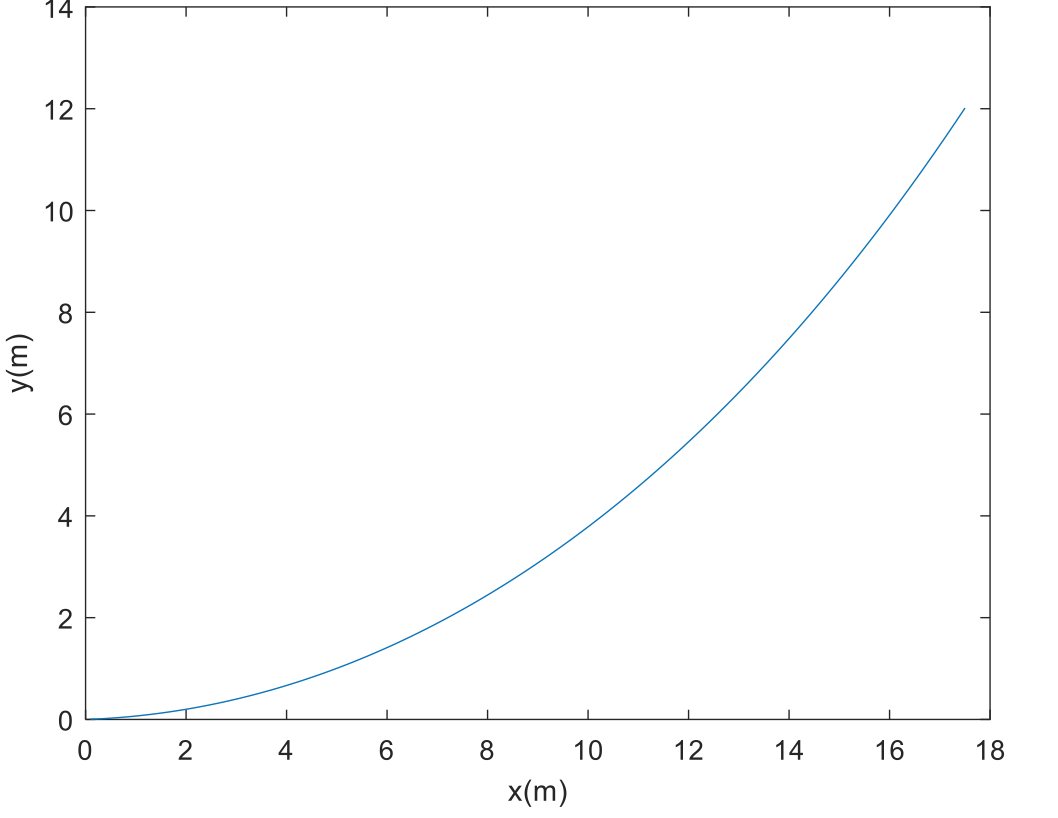
\includegraphics[width=12cm]{q1-24-2.png}
\caption{风速为$24m/s$时锚链形状拟合曲线} \label{fig:q1-24-2}
\end{figure}

\newpage
\subsubsection{求解结果汇总}
在$12m/s$和$24m/s$两种风速下,通过计算得到系泊系统的参数如下表(\ref{q1-ans-table},\ref{q1-ans-table2})所示。其中第一节锚链环指沿$x$轴正方向不沉于海床面的第一节锚链环。
\begin{table}[!htbp]
\centering
\caption{已知风速和钢球质量条件下系泊系统模型计算结果}
\label{q1-ans-table}
\begin{tabular}{cccccccccc}
\toprule
风速(m/s)& 吃水深度(m)& 游动半径(m)& 钢桶倾角(度)& 第一节锚链环的$\theta$(度) \\
\midrule
12 & 0.73072 & 14.5085 & 1.0217 & 0 \\
24 & 0.74432 & 18.8359 & 3.9062 & 2.1329 \\ 
\bottomrule 
\end{tabular}
\end{table}

\begin{table}[!htbp]
\centering
\caption{不同风速下每节钢管与x轴的夹角}
\label{q1-ans-table2}
\begin{tabular}{cccccccccc}
\toprule
风速(m/s)& 第1节钢管(°)& 第2节钢管(°)& 第3节钢管(°)& 第4节钢管(°) \\
\midrule
12 &88.99203281	&88.99807116	&89.00403761	&89.00993342\\
24 &86.14437348	&86.16667411	&86.18871863	&86.21051143\\
\bottomrule 
\end{tabular}
\end{table}

\newpage
\section{风速为$36m/s$时系泊系统优化模型}
\subsection{模型建立}      

\par 在已知风速和和钢球质量条件下的系泊系统计算模型的基础上,通过调节重物球的质量,使得钢桶的倾斜角度不超过5度,锚链在锚点与海床的夹角不超过16度。建立非线性规划模型,确定金属球的最小质量。
\subsubsection{非线性规划模型}
由于金属球的质量直接影响钢桶与锚链的倾斜角度,为了保证通讯质量,确定该规划的约束为钢桶的倾角小于 ,第一节锚链的倾斜角度小于 ;以及锚链、钢桶、钢管在竖直方向上的投影长度与浮标吃水深度 之和为海水深度18米。建立非线性规划目标如公式(\ref{q2-guihua-1})所示。由于海风风速为$24m/s$时所有锚链环已完全浮于海水中,因此在海风风速为$36m/s$时,参与计算的锚链环个数为210个。
$$
min \quad m_B
$$
\begin{equation}
	\label{q2-guihua-1}
	s.t.\left\{
	\begin{split}
		& \sum\limits_{i=1}^{4} l_P sin\theta_{Pi} + l_D sin\theta_D + \sum\limits_{i=1}^{210} l_A sin \theta_{Ai} + h = 18 \\
		& 0^o \leqslant \theta_D \leqslant 16^o \\
		& 0^o \leqslant \theta_{A1} \leqslant 5^o \\
	\end{split}	
	\right.
\end{equation}

\subsection{模型求解}
\par 利用已知风速和和钢球质量条件下的系泊系统计算模型,解得在重物球质量仍为$1200kg$、风速为$36m/s$时,各项参数(如表(\ref{q2-ans-table0})所示)均不符合题目要求,因此通过搜索确定所需要的重物球最小质量。
\begin{table}[!htbp]
\centering
\caption{风速为$36m/s$、钢桶重量为$1200kg$时的结果}
\label{q2-ans-table0}
\begin{tabular}{cccccccccc}
\toprule
重物球质量(Kg)& 吃水深度(m)& 游动半径(m)& 钢桶倾角(度)& 第一节锚链环的$\theta$(度) \\
\midrule
1200 & 0.77 & 18.2354 & 8.1834 & 19.3025\\
\bottomrule 
\end{tabular}
\end{table}

\par 假定重物球质量在$3000kg$以内,首先对重物球质量在$1200kg$到$3000kg$的范围内按步长为$100kg$进行搜索,约束条件为$h \in (0.76,2)$得到在重物球质量为$3000kg$时,浮标吃水深度$h$为$1.260$米,符合条件。
3000	1.26000000000000	
\par 后将搜索范围缩小至$2900kg$到$3100kg$,进行步长为$10kg$的搜索,约束条件$h \in (1.16,1.36)$,得到在重物球质量为$2900kg$时,浮标吃水深度$h$为$1.230$米,结果更优。

\par 再次细化搜索范围到$2890kg$到$2910kg$之间进行步长为$1kg$的搜索,约束条件$h \in (1.22,1.24)$,得到重物球质量为$2890kg$时,浮标吃水深度为$1.23$米,得到最终结果如下表(\ref{q2-ans-table},\ref{q2-ans-table2})所示。

\begin{table}[!htbp]
\centering
\caption{风速为$36m/s$时系泊系统优化模型}
\label{q2-ans-table}
\begin{tabular}{cccccccccc}
\toprule
重物球质量(Kg)& 吃水深度(m)& 游动半径(m)& 钢桶倾角(度)& 第一节锚链环的$\theta$(度) \\
\midrule
2890 & 1.23 & 19.4888 & 4.0093 & 15.0641\\
\bottomrule 
\end{tabular}
\end{table}

\begin{table}[!htbp]
\centering
\caption{风速为$36m/s$时每节钢管与x轴的夹角}
\label{q2-ans-table2}
\begin{tabular}{cccccccccc}
\toprule
第1节钢管(°)& 第2节钢管(°)& 第3节钢管(°)& 第4节钢管(°) \\
\midrule
86.02162275	&86.0353563	&86.04899551	&86.06254134\\
\bottomrule 
\end{tabular}
\end{table}

得到系泊系统中各个组件的位置如下图(\ref{fig:q2-36-1})所示。
\begin{figure}[h]
\small
\centering
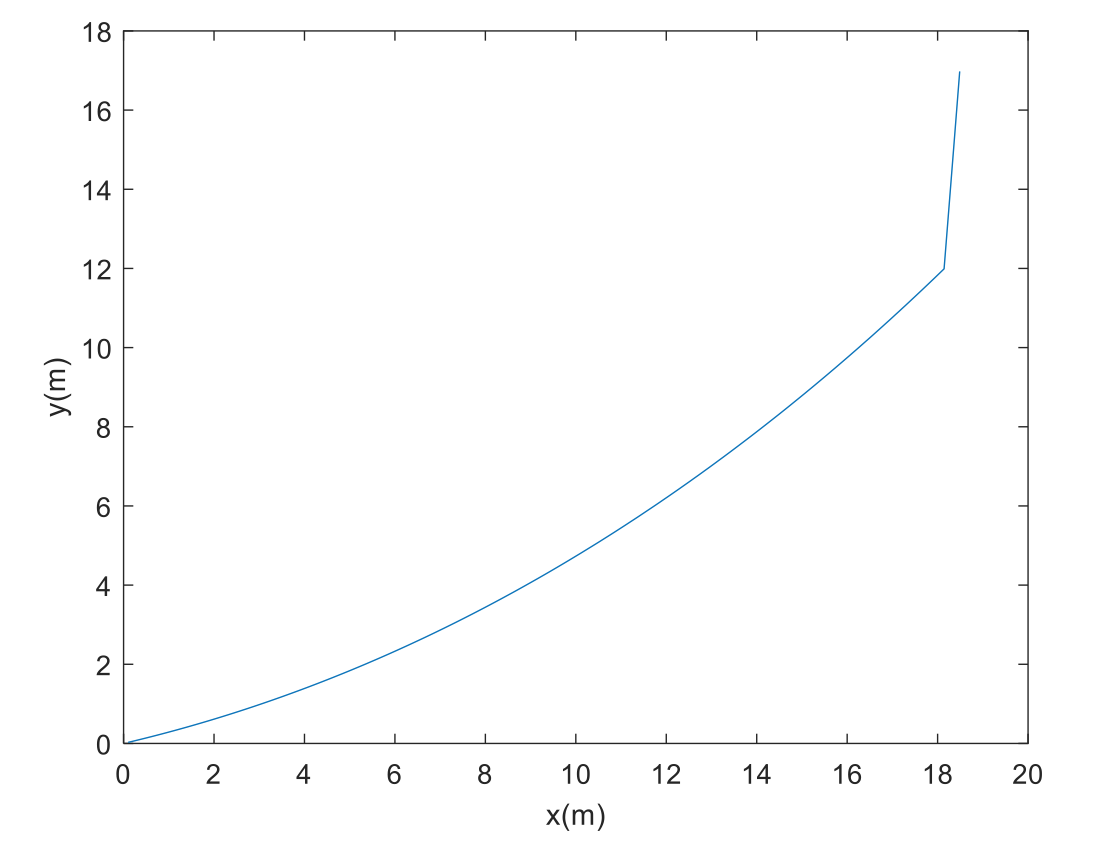
\includegraphics[width=12cm]{q2-36-1.png}
\caption{风速为$36m/s$时系泊系统各组件位置} \label{fig:q2-36-1}
\end{figure}
对锚链形状曲线进行拟合,得到结果如下公式(\ref{q2-ans-1})所示。其拟合曲线如图(\ref{fig:q2-36-2})所示。经检验,拟合结果误差在$10^{-5}$数量级以内,可保证结果有效。
\begin{equation}
	\label{q2-ans-1}
	y = 0.0000027x^4+0.000057x^3+0.019x^3+0.27x^2+0.000098 \quad  (0<x<18.14)
\end{equation}

\begin{figure}[h]
\small
\centering
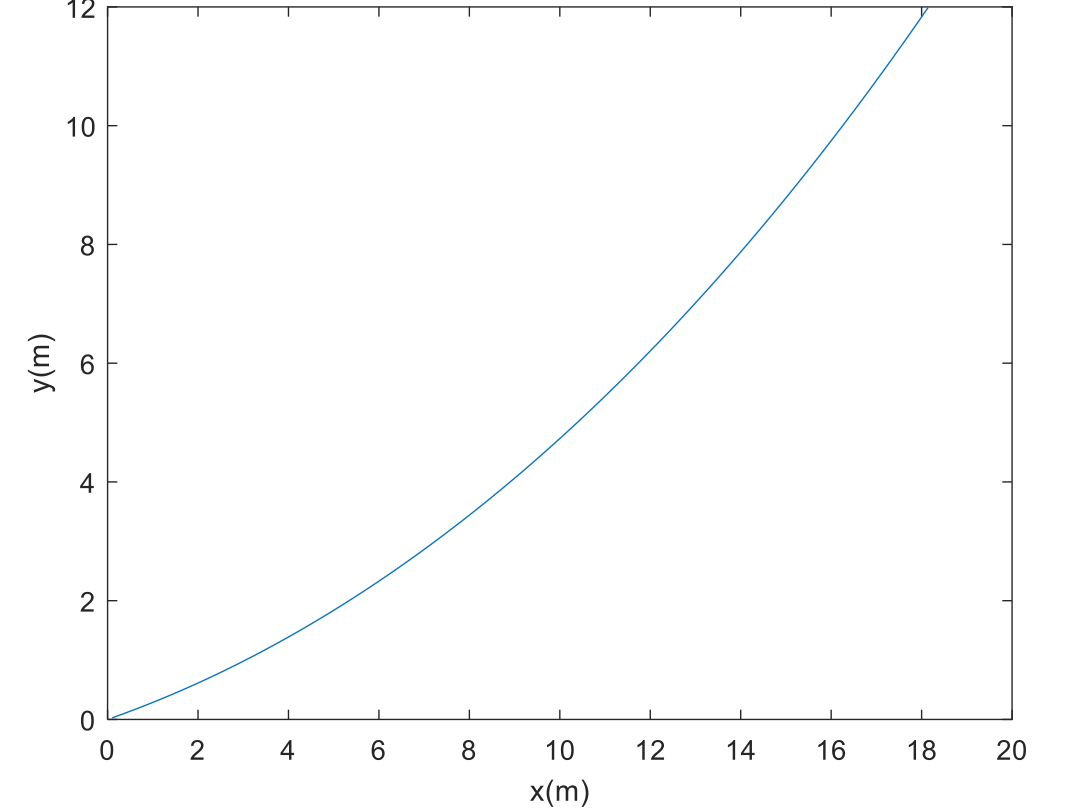
\includegraphics[width=12cm]{q2-36-2.png}
\caption{风速为$36m/s$时锚链形状拟合曲线} \label{fig:q2-36-2}
\end{figure}



\newpage
\section{风力、水流力和水深综合影响下系泊系统优化模型}

\subsection{模型建立}
\par 以锚为坐标原点,沿海床平面水平向右为$x$轴正方向,竖直向上方向为$y$轴正方向建立直角坐标系(如下图()所示为建立的坐标系及受力分析)。在已知风速和和钢球质量条件下的系泊系统计算模型的基础上,进行分析。
\begin{figure}[h]
\small
\centering
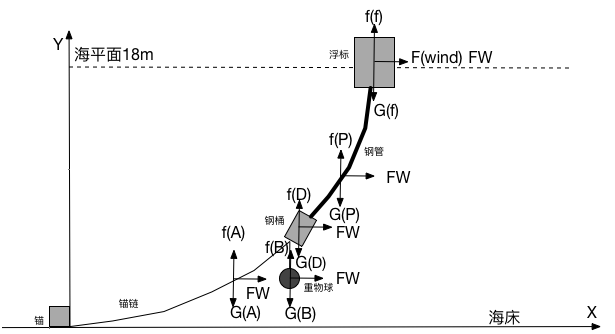
\includegraphics[width=10cm]{zuobiaoxi2.png}
\caption{坐标系建立及受力分析} \label{fig:zuobiaoxi2}
\end{figure}

\subsubsection{根据几何关系建立各组件重心与倾角关系}
\par 由几何关系得到系统中各个部件重心位置和部件与海平面间夹角的几何关系式组(\ref{weiyifangcheng-2})如下所示。
\begin{equation}
	\label{weiyifangcheng-2}
	\left\{
	\begin{array}{lr}
		x_{Ak} = \frac{l_A}{2} cos \theta_{Ak} + \sum\limits_{i=1}^{k-1} l_A cos \theta_{Ai}\\
		x_B = \sum\limits_{i=1}^{n} l_A cos \theta_{Ai}\\
		x_D = \frac{l_D}{2} cos \theta_D + \sum\limits_{i=1}^{n} l_A cos \theta_{Ai}\\
		x_{Pj} = \frac{l_P}{2} cos \theta_{Pj} + \sum\limits_{i=1}^{j-1} l_P cos \theta_{Pi} + l_D cos \theta_D + \sum\limits_{i=1}^{n} l_A cos \theta_{Ai} \quad j = 1,2,3,4 \\
		x_f = \sum\limits_{i=1}^{4} l_P cos \theta_{Pi} + l_D cos \theta_D + \sum\limits_{i=1}^{n} l_A cos \theta_{Ai} + \frac{1}{2} d_f + (N - n) \cdot l_A\\
		y_{Ak} = \frac{l_A}{2} sin \theta_{Ak} + \sum\limits_{i=1}^{k-1} l_A sin \theta_{Ai}\\
		y_B = \sum\limits_{i=1}^{n} l_A sin \theta_{Ai}\\
		y_D = \frac{l_D}{2} sin \theta_D + \sum\limits_{i=1}^{n} l_A sin \theta_{Ai}\\
		y_{Pj} = \frac{l_P}{2} sin \theta_{Pj} + \sum\limits_{i=1}^{j-1} l_P sin \theta_{Pi} + l_D sin \theta_D + \sum\limits_{i=1}^{n} l_A sin \theta_{Ai} \quad j = 1,2,3,4 \\
		y_f = \sum\limits_{i=1}^{4} l_P sin \theta_{Pi} + l_D sin \theta_D + \sum\limits_{i=1}^{n} l_A sin \theta_{Ai} + \frac{1}{2} L_f\\
	\end{array}
	\right.
\end{equation}

\subsubsection{各部件所受主动力的分析}
\par 由于海水中存在着流速度,因此系泊系统中各个组件会受到近海水流力的影响,该力可由公式(\ref{q3-fw})所示方法求得。其中$\mu$为近海水流速度,$S$为水流方向上部件面积的投影。
\begin{equation}
	\label{q3-fw}
	FW = 374 \times S \times \mu^2 
\end{equation}
\par 因此在使用虚功原理时,需要考虑水平近海水流力及其对应的虚位移。公式组(\ref{weiyifangcheng-2})中,$x_{Ak}$为第$k$个锚链链环重心所在位置对应的横坐标;$x_D$为钢桶重心所在位置对应的横坐标;$x_{Pj}$为第$j$根钢管重心所在位置的横坐标;$x_B$为钢球重心所在位置的横坐标;$x_f$为浮标重心所在位置对应的横坐标。
 
\subsubsection{基于虚功原理的优化模型}
\par 由前述受力与虚位移几何关系分析,根据虚功原理建立方程(\ref{q3-xugongyuanli})。
\begin{equation}
	\label{q3-xugongyuanli}
	\begin{split}
		0 &= \sum\limits_{k=1}^{n} P_A \cdot \delta y_{Ak} + P_D \cdot \delta y_{D} + \sum\limits_{j=1}^{4} P_P \cdot \delta y_{Pj} + P_B \cdot \delta y_{B} + P_f \cdot \delta y_{f} + \sum\limits_{k=1}^{n} FW_A \cdot \delta x_{Ak} \\
		& +  FW_D \cdot \delta x_{D} + \sum\limits_{j=1}^{4} FW_P \cdot \delta x_{Pj} +  (F_{wind} + FW_f) \cdot \delta x_{f}		
	\end{split}
\end{equation}
\par 根据前述几何关系分析、受力分析以及虚功原理方程可解得如下公式组(\ref{q3-ans-1})中所示系泊系统中各个部件与海平面间夹角的正切值。其中$\theta_{Ak}$、$\theta_{D}$、$\theta_{Pj}$表示第$k$节锚链链环与水平方向的夹角、钢桶轴线与水平方向的夹角和第$j$节钢管与水平方向的夹角。
\begin{equation}
	\label{q3-ans-1}
	\left\{
	\begin{array}{lr}
        tan\theta_{Ak} = \frac{(n+\frac{1}{2} - k)P_A +P_D+4P_P+P_B+P_f}{[(n+\frac{1}{2} - k)FW_A +FW_D+4FW_P+FW_f] + F_{wind}} \\
        tan\theta_{D} = \frac{\frac{1}{2}P_D+4P_P+P_f}{(\frac{1}{2}FW_D+4FW_P+FW_f)+F_{wind}}\\
        tan\theta_{Pj} = \frac{(4.5-j)P_P+P_f}{(4.5-j)FW_P+FW_f+F_{wind}}
	\end{array}
	\right.
\end{equation}
\par 近浅海观测网的传输节点中首先需要保证水声设备工作效果最优;其次要保证浮标吃水深度较浅,以便于数据传输和检查;最后要使得浮标游动区域尽可能小,以确保数据采集的稳定性。因此,我们建立分层优化模型如下公式(\ref{q3-ans-3})所示。公式中n为锚链浮于水中的锚链环的节数。
\[
	\begin{split}
		&min \quad \theta_D \\
		&\qquad min \quad h \\
		&\qquad \qquad min \quad R\\
	\end{split}
\]
\begin{equation}
	\label{q3-ans-3}
	\left\{
	\begin{split}
		& 190 \leqslant n \leqslant 230\\
		& 19 \leqslant \sum\limits_{i=1}^{4}l_P sin \theta_{Pi} + l_D sin \theta_{D} + \sum\limits_{i=1}^{n} l_A sin \theta_{Ai} + h \leqslant 20\\
		& \theta_{A1} \leqslant 16^o \\
		& \theta_{D} \leqslant 5^o \\
		& 0 < h \leqslant 2\\
	\end{split}
	\right.
\end{equation}


\subsection{模型求解}
\par 第三问中需要整体考虑在风力、水流力和水深情况下的系泊系统设计。本文将该问题分为两步:
\begin{enumerate}
	\item 考虑极端条件下(海水速度为$1.5m/s$、风速为$36m/s$、海风速同向、水深为$19\sim 20m$)选用不同型号锚链,得到钢桶、钢管的倾斜角度、锚链形状、浮标的吃水深度和游动区域。然后以最优钢桶的倾斜角度(与垂直方向夹角越小越好),次优浮标的吃水深度(吃水深度越浅越好),再次优浮标的游动区域(游动区域越小越好)为原则,选出最优的锚链型号。
	\item 对于最优的锚链型号,分别分析不同水深、不同海水速度、不同风速下钢桶、钢管的倾斜角度、锚链形状、浮标的吃水深度和游动区域。
\end{enumerate}

\subsubsection{锚链型号选择}
一个好的锚链,需要承受住极端条件的考研。本文需要先分别对5种锚链型号在极端条件下进行分析,从而选出最优的锚链。对一种锚链型号来说,将极端条件(海水速度为$1.5m/s$、风速为$36m/s$、海风速同向、水深为$19\sim 20m$)作为条件,变动重物球的质量、吃水深度、锚链链环节数,将钢桶的倾斜角度、第1节锚链与海平面夹角、整个系泊系统在竖直方向投影长度作为约束,从而得到满足条件的解,具体求解算法步骤如下:
\begin{enumerate}
	\item 以第二问求解出的重物球质量$2890kg$作为搜索下限,$20000kg$作为搜索上限,步长为$100kg$。
	\item 对于链环节数,以第一问的$210$节为参考,将$190$节作为搜索下限,$230$节作为搜索上限,步长为$1$节。
	\item 对于吃水深度,以$0m$作为搜索下限,$2m$作为搜索上限,步长为$0.01m$。
	\item 判断是否同时满足钢桶与垂直方向角度小于$5°$,第 1 节锚链与海平面夹角小于$16°$,整个系泊系统在竖直方向投影长度在$19\sim 20m$,若同时满足则停止搜索,返回此时的重物球的质量、吃水深度、锚链链环节数,并计算出对应的钢桶、钢管的倾斜角度和游动区域并绘制出锚链形状,否则继续搜索。
\end{enumerate}


\begin{table}[!htbp]
\centering
\caption{系泊系统用不同型号锚链在极端条件下的参数}
\label{q3-ans-table1}
\begin{tabular}{lccccccccc}
\toprule
锚链型号 & I & II & III & IV & V \\
\midrule
链环节数	&224&224&224&224&225\\ 
锚链长度	& 17.472&23.52&26.88&33.6&40.5\\
重物球质量(kg) &6500&8900&11600&15200&19100\\
吃水深度(m)	&1.13&1.03&1.03&1.04&1.03\\
游动半径(m)	&19.3267&19.3394&19.3388&19.3169&19.4387\\
钢桶倾斜角度(°)	& 3.9305&4.8999&4.8999&4.7909&4.8999\\
第1节锚链与海平面夹角(°)&15.9727&15.9923&15.9390&15.9946&15.9603\\
\bottomrule 
\end{tabular}
\end{table}

\par 根据表格(\ref{q3-ans-1}),可以发现在以最优钢桶的倾斜角度(与垂直方向夹角越小越好),次优浮标的吃水深度(吃水深度越浅越好),再次优浮标的游动区域(游动区域越小越好)为原则,选出最优的锚链型号为$I$。而且可以发现,在相同的约束条件下,不同型号游动半径、吃水深度变化不大,$I$的钢桶与垂直方向角度最小而且I用到的重物球质量仅为$6500kg$,毫无疑问是最优的。

\subsubsection{不同风力、水流力和水深的影响}

\par 选定锚链I后,即需要分析不同水深、不同海水速度、不同风速对的影响。沿用选定锚链$I$确定下的数据,链环节数为$224$,重物球质量为$6500$。

\textbf{不同风力对系泊系统的影响钢桶、钢管的倾斜角度、锚链形状、浮标的吃水深度和游动区域}
\par 将海水速度定为$1.5m/s$,水深定为$20m$(具体做法为变动吃水深度使整个系泊系统在竖直方向投影长度为$20m$),分别考虑风速为$12m/s$,$24m/s$和$36m/s$时,风力对系泊系统参数(钢桶、钢管的倾斜角度和游动区域)的影响如表(\ref{q3-ans-table2})所示,并绘制出锚链形状(如图(\ref{fig:q3-fengsu})所示)。

\begin{table}[!htbp]
\centering
\caption{水深$20m$水速$1.5m/s$时不同风速下系泊系统的参数}
\label{q3-ans-table2}
\begin{tabular}{lccccccccc}
\toprule
风速($m/s$)&12&24&36\\
\midrule
钢桶倾斜角度(°)&1.4684&3.1694&6.3372\\
第1节钢管与海平面夹角(°)&1.4684&3.1694&6.3372\\
第2节钢管与海平面夹角(°)&89.0754&87.4119&84.3097\\
第3节钢管与海平面夹角(°)&89.1954&87.5420&84.4578\\
第4节钢管与海平面夹角(°)&89.3145&87.6710&84.6047\\
第1节锚链与海平面夹角(°)&18.0727&18.2429&18.4775\\
吃水深度(m)&0.97&0.95&0.92\\
游动半径(m)&18.2784&18.4404&18.7557\\
\bottomrule 
\end{tabular}
\end{table}

\begin{figure}[h]
\small
\centering
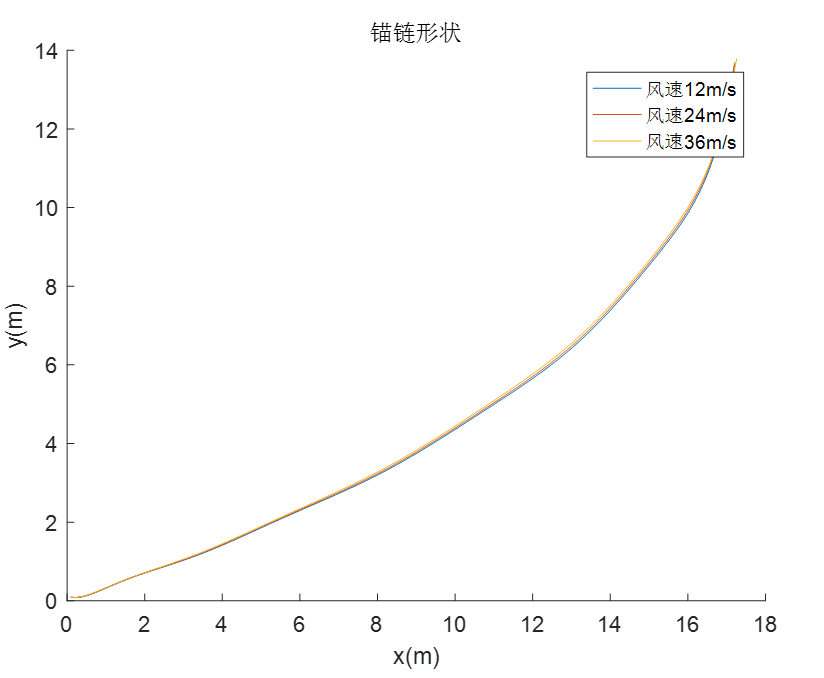
\includegraphics[width=12cm]{q3-fengsu.png}
\caption{水深$20m$水速$1.5m/s$时不同风速下的锚链形状} \label{fig:q3-fengsu}
\end{figure}

\newpage
\textbf{不同水流力对系泊系统的影响}
\par 将风速定为$18m/s$, 水深定为$20m$(具体做法为变动吃水深度使整个系泊系统在竖直方向投影长度为$20m$),分别考虑海水速度为$0.3m/s$,$0.6m/s$、$0.9m/s$、$1.2m/s$和$1.5m/s$时,不同水流力对系泊系统参数(钢桶、钢管的倾斜角度和游动区域)的影响如表(\ref{q3-ans-table3})所示,并绘制出锚链形状(如图(\ref{fig:q3-shuisu})所示)。


\begin{table}[!htbp]
\centering
\caption{风速$18m/s$水深$20m$时不同水速下系泊系统的参数}
\label{q3-ans-table3}
\begin{tabular}{lccccccccc}
\toprule
水速($m/s$)&0.3&0.6&0.9&1.2&1.5\\
\midrule
钢桶倾斜角度(°)&2.2177&1.8955&2.0279&2.2400&2.4669\\
第1节钢管与海平面夹角(°)&87.8353&88.2085&88.1742&88.0926&88.0161\\
第2节钢管与海平面夹角(°)&87.8548&88.2409&88.2342&88.1894&88.1554\\
第3节钢管与海平面夹角(°)&87.8740&88.2731&88.2937&88.2854&88.2935\\
第4节钢管与海平面夹角(°)&87.8929&88.3049&88.3526&88.3805&88.4304\\
第1节锚链与海平面夹角(°)&87.2118&80.1954&68.5784&51.6388&25.3442\\
吃水深度(m)&0.75&0.83&0.85&0.87&0.90\\
游动半径(m)&8.5499&9.3993&10.7702&12.7116&16.6002\\
\bottomrule 
\end{tabular}
\end{table}

\begin{figure}[h]
\small
\centering
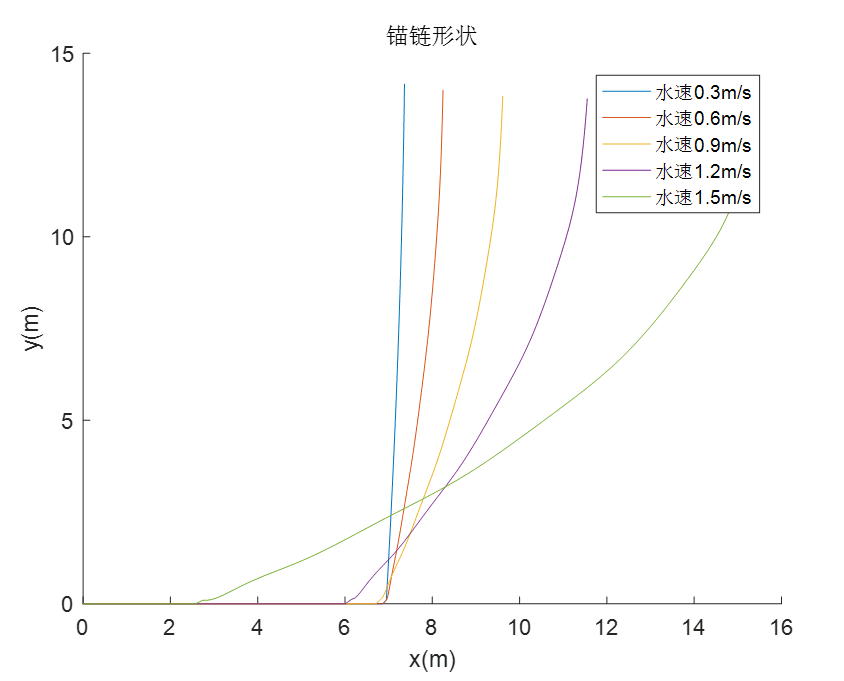
\includegraphics[width=12cm]{q3-shuisu.png}
\caption{风速$18m/s$水深$20m$时不同水速下的锚链形状} \label{fig:q3-shuisu}
\end{figure}

\textbf{不同水深对系泊系统的影响}
\par 将风速定为$36m/s$, 海水速度定为$1.5m/s$,分别考虑水深为$16m$、$17m$、$18m$、$19m$和$20m$(具体做法为变动吃水深度使整个系泊系统在竖直方向投影长度为给定水深),不同水深对系泊系统参数(钢桶、钢管的倾斜角度和游动区域)的影响如表(\ref{q3-ans-table4})所示,并绘制出锚链形状(如图(\ref{fig:q3-shuishen})所示)。


\begin{table}[!htbp]
\centering
\caption{风速$36m/s$水速$1.5m/s$时不同水深下系泊系统的参数}
\label{q3-ans-table4}
\begin{tabular}{lccccccccc}
\toprule
水深(m)&16&17&18&19&20 \\
\midrule
钢桶倾斜角度(°)&1.4358&1.9799&2.7357&3.9305&6.3372\\
第1节钢管与海平面夹角(°)&88.7806&88.2658&87.5517&86.4244&84.1605\\
第2节钢管与海平面夹角(°)&88.8430&88.3370&87.6354&86.5289&84.3097\\
第3节钢管与海平面夹角(°)&88.9051&88.4078&87.7187&86.6328&84.4578\\
第4节钢管与海平面夹角(°)&88.9670&88.4784&87.8076&86.7360&86.6047\\
第1节锚链与海平面夹角(°)&10.2263&12.0098&13.8882&15.9727&18.4475\\
吃水深度(m)&4.59&1.45&1.3&1.13&0.92\\
游动半径(m)&20.9760&20.4301&19.8853&19.3266&18.7557\\
\bottomrule 
\end{tabular}
\end{table}


\begin{figure}[h]
\small
\centering
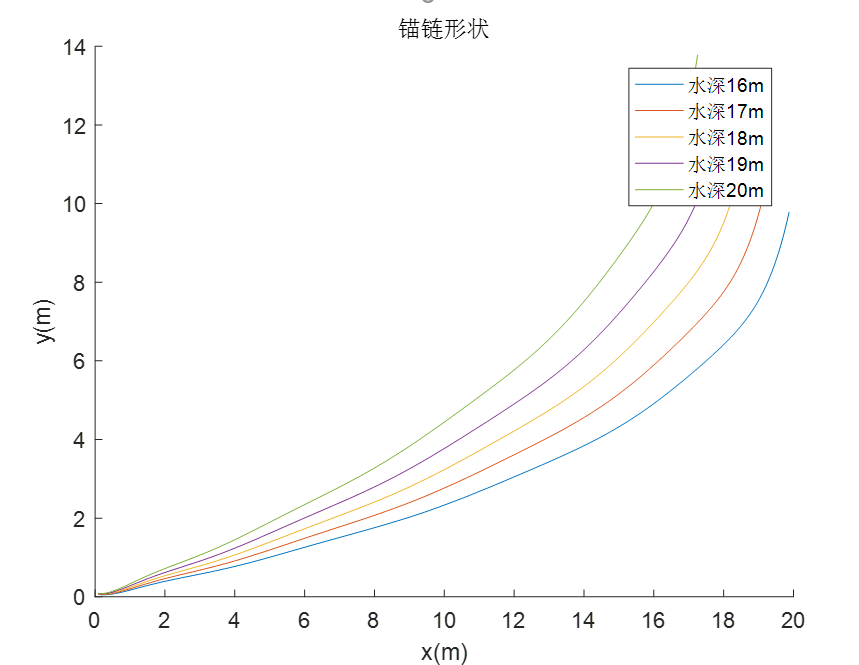
\includegraphics[width=12cm]{q3-shuishen.png}
\caption{风速$36m/s$水速$1.5m/s$时不同水深下的锚链形状} \label{fig:q3-shuishen}
\end{figure}



\newpage
\newpage

\section{模型优缺点}
\subsection{模型优点}
\begin{enumerate}
	\item 本文使用分析力学的方法,将锚链精确到每一个锚链链环,对模型的刻画符合实际情况,模型刻画精度高。
	\item 牛顿力学对每一个倾角需要使用迭代的方法,而本文采用分析力学虚功原理解释理想约束的平衡问题时,由于约束反力自动消去,可以简单的用它去求主动力在平衡时所满足的条件,即平衡条件,倾角之间是彼此相互独立的,省去了迭代步骤。
\end{enumerate}
\subsection{模型缺点}
本文在分析浮标的吃水深度时,我们假定浮标的轴线与海平面垂直,却没有考虑浮标实际情况是会在风载荷作用下倾斜的情形。
\section{模型改进方向}
\par 本文在进行模型分析时,假定浮标的轴线与海平面垂直,而实际的情况,在风载荷的作用下会产生一个倾角,因此在模型改进中,本文需要将这一情形纳入考虑。

%参考文献
\begin{thebibliography}{9}%宽度9
 \bibitem{理论力学} 蔡泰信, 和兴锁, 朱西平. 理论力学[M]. 机械工业出版社, 2007.
 \bibitem{浮标} https://baike.baidu.com/item/海洋浮标/9246083?fr=aladdin
\end{thebibliography}
\newpage
\appendix
\section{程序}
cpp\textcolor[rgb]{0.98,0.00,0.00}{\textbf{Input C++ source:}}
% 代码插入,请将代码文件放入code文件夹,支持语言的语法高亮。支持语言:C,C++,Java,Matlab,Mathematica,python,R,可在cls文件中自行添加。
\lstinputlisting[language=C++]{./code/a.cpp}


\end{document}